\documentclass[a4paper,10pt,titlepage]{report}

\usepackage[utf8]{inputenc}
\usepackage[T1]{fontenc}
\usepackage[english]{babel}
\usepackage{amssymb}
\usepackage{amsmath}
\usepackage{amsthm}
\usepackage{graphicx}
\usepackage{fancyhdr}
\usepackage{lastpage}
\usepackage{listings}
\usepackage{algorithm}
\usepackage{algpseudocode}
\usepackage[document]{ragged2e}
\usepackage[margin=1in]{geometry}
\usepackage{enumitem}
\usepackage{color}
\usepackage{datenumber}
\usepackage{venndiagram}
\usepackage{chngcntr}
\usepackage{mathtools}
\usepackage{booktabs}


\DeclarePairedDelimiter{\ceil}{\lceil}{\rceil}

%lstlisting ting:
\definecolor{dkgreen}{rgb}{0,0.45,0}
\definecolor{gray}{rgb}{0.5,0.5,0.5}
\definecolor{mauve}{rgb}{0.30,0,0.30}
\lstset{frame=tb,
  language=C,
  aboveskip=3mm,
  belowskip=3mm,
  showstringspaces=false,
  columns=flexible,
  basicstyle={\small\ttfamily},
  numbers=left,
  numberstyle=\footnotesize,
  keywordstyle=\color{dkgreen}\bfseries,
  commentstyle=\color{dkgreen},
  stringstyle=\color{mauve},
  frame=single,
  breaklines=true,
  breakatwhitespace=false
  tabsize=1
}
\lstset{literate=%
{æ}{{\ae}}1
{å}{{\aa}}1
{ø}{{\o}}1
{Æ}{{\AE}}1
{Å}{{\AA}}1
{Ø}{{\O}}1
}
\lstset{extendedchars=\true}
\lstset{inputencoding=ansinew}
\renewcommand{\lstlistingname}{Code} 

\setdatetoday
\addtocounter{datenumber}{0} %date for dilierry standard is today
\setdatebynumber{\thedatenumber}
\date{}



\setcounter{section}{-1}

\setcounter{tocdepth}{3}
\setcounter{secnumdepth}{-1}

\pagestyle{fancy}
\fancyhf{}
\title{CC - Assignment 3}

\newcommand{\Z}{\mathbb{Z}}
\lhead{Compiler (DM546)}
\rhead{Mjerv15, Trpet15  \& Mojae15}
\rfoot{Page  \thepage \, of \pageref{LastPage}}
\counterwithin*{equation}{section}

\begin{document}
\newpage
{%
\centering
    \huge
    \bfseries
    \vspace{5mm}
CC, Spring 2018\\
Exam project, part 3\\
\vspace{5mm}
\begin{tabular}{|l|l|}
\hline
Group & 1 \\ \hline
\end{tabular}
\\
\vspace{10mm}
\begin{tabular}{@{}ll@{}}
\toprule
\multicolumn{1}{|l|}{Name}      & \multicolumn{1}{l|}{Mark Wolff Jervelund } \\ \midrule
\multicolumn{1}{|l|}{Birthday}  & \multicolumn{1}{l|}{280795} \\ \midrule
\multicolumn{1}{|l|}{Login}     & \multicolumn{1}{l|}{mjerv15@student.sdu.dk} \\ \midrule
\multicolumn{1}{|l|}{Signature} & \multicolumn{1}{l|}{\includegraphics[scale=0.3]{../img/mark_sign}} \\ \midrule
                                &                       \\ \midrule
\multicolumn{1}{|l|}{Name}      &  \multicolumn{1}{l|}{Troels Blicher Petersen} \\ \midrule
\multicolumn{1}{|l|}{Birthday}      &   \multicolumn{1}{l|}{230896} \\ \midrule
\multicolumn{1}{|l|}{Login}      &  \multicolumn{1}{l|}{trpet15@student.sdu.dk} \\ \midrule
\multicolumn{1}{|l|}{Signature}      & \multicolumn{1}{l|}{\includegraphics[scale=0.08]{../img/troels_sign} } \\ \midrule
                                &                       \\ \midrule
\multicolumn{1}{|l|}{Name}     &  \multicolumn{1}{l|}{Morten Kristian Jæger} \\ \midrule
\multicolumn{1}{|l|}{Birthday}      &  \multicolumn{1}{l|}{030895} \\ \midrule
\multicolumn{1}{|l|}{Login}     &   \multicolumn{1}{l|}{mojae15@student.sdu.dk} \\ \midrule
\multicolumn{1}{|l|}{Signature}    &  \multicolumn{1}{l|}{\includegraphics[scale=0.3]{../img/morten_sign}} \\ \midrule
\end{tabular}
\\
\vspace{10mm}
This report contains a total of \underline{ \pageref{LastPage} } pages.
}

\begin{titlepage}
\centering
    \vspace*{9\baselineskip}
    \huge
    \bfseries
    3. Assignment \\
    \normalfont 
    Mark Jervelund, Troels Blicher Petersen \& Morten Jæger  \\
    (Mjerv15, Trpet15, Mojae15) \\
	\huge    
    Compiler (DM546)  \\[4\baselineskip]
    \normalfont
	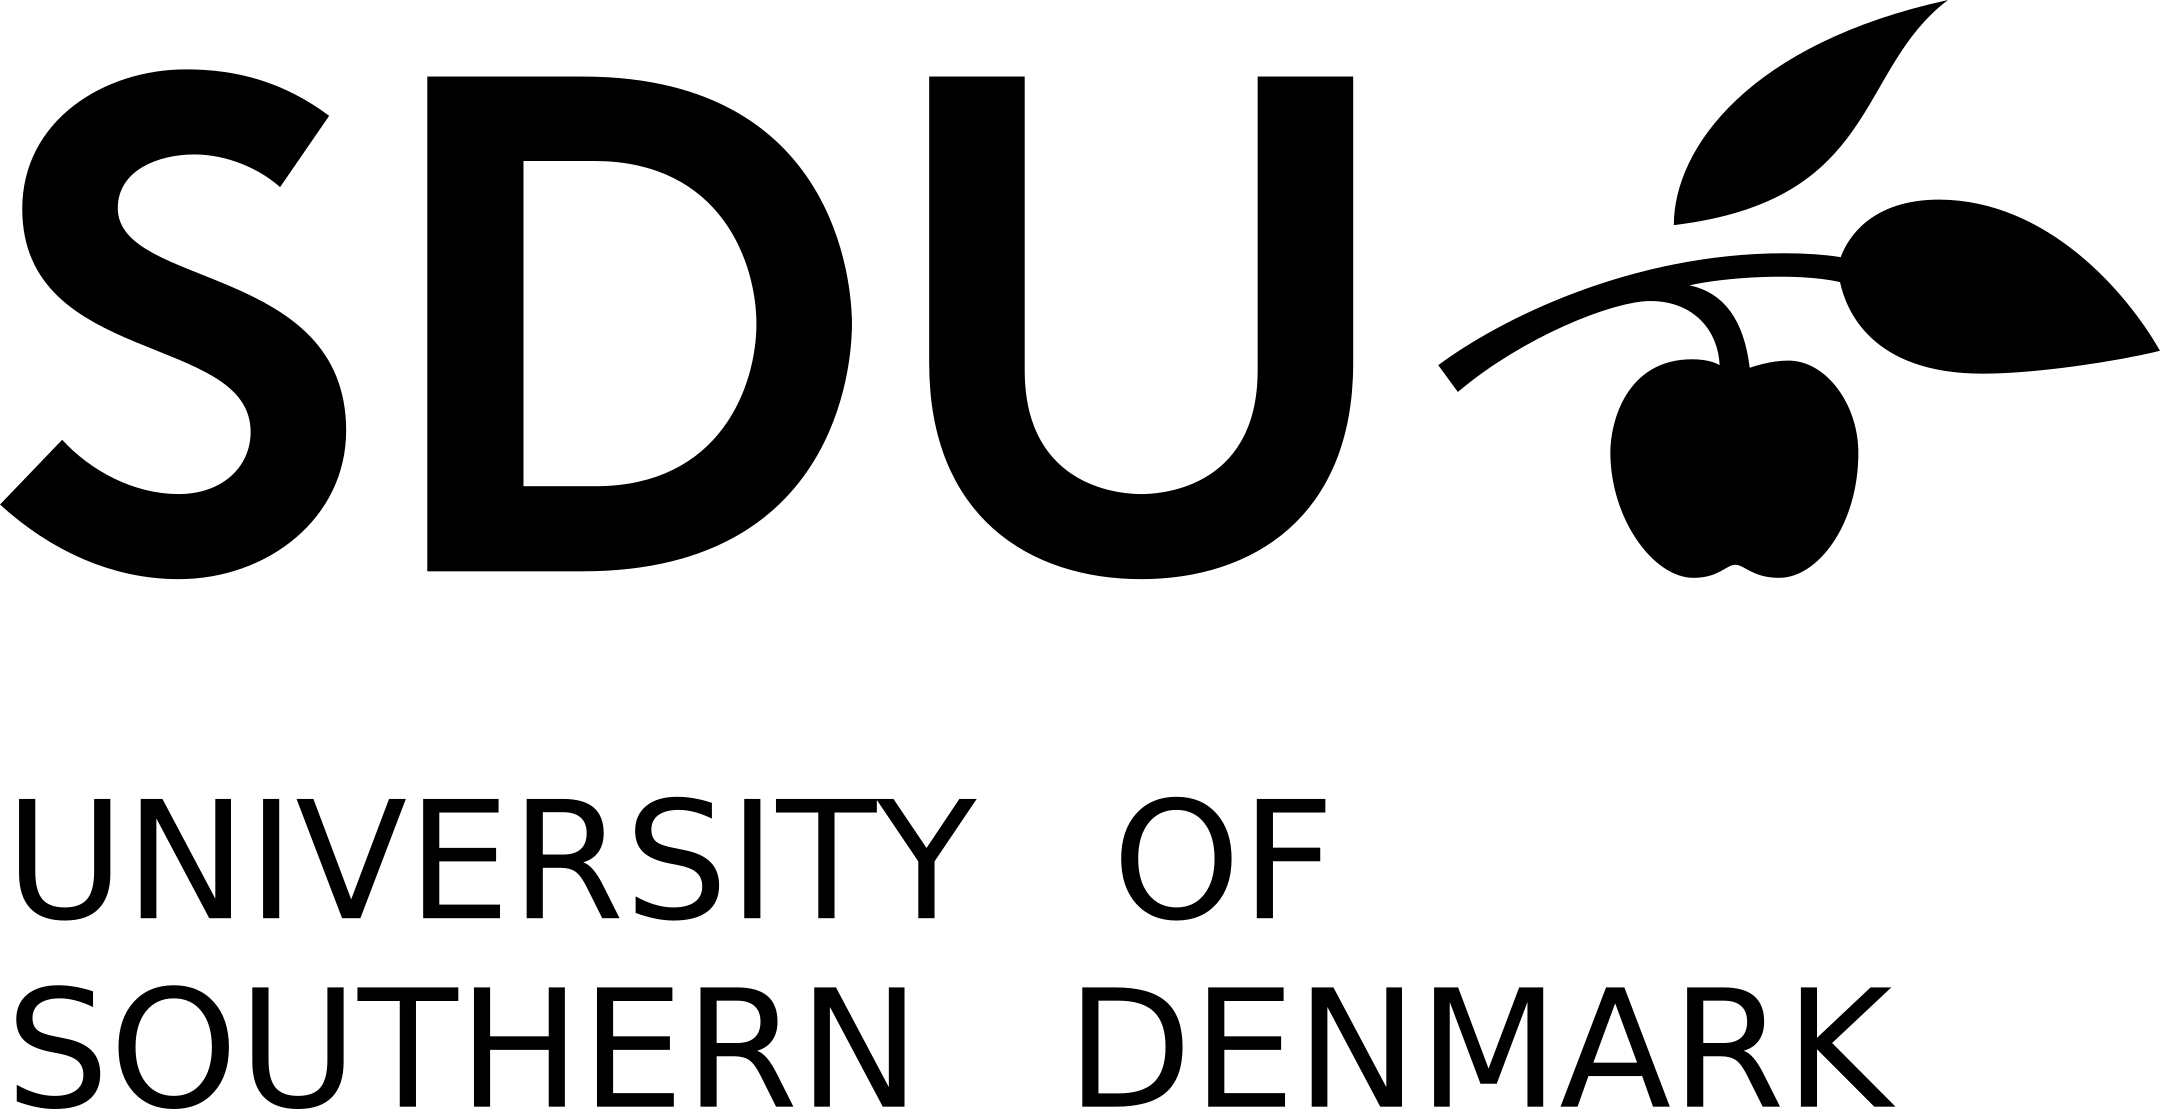
\includegraphics[scale=1]{../img/SDU_logo}
    \vfill\ 
    \vspace{5mm}
    IMADA \\

    \textbf{\datedate} \\[2\baselineskip]
\end{titlepage}

\renewcommand{\thepage}{\roman{page}}% Roman numerals for page counter
\tableofcontents
\newpage
\setcounter{page}{1}
\renewcommand{\thepage}{\arabic{page}}
\newpage

\section{Introduction}
In the third assignment of the Compiler project, we are tasked with implementing a weeder phase and a typechecking phase, with primary focus on the typechecking phase. This entire third assignment in made only in C.

\subsection{Build and execute}
To build and execute first run either \textsf{make}, \textsf{make all} or \textsf{make compiler}.
\begin{lstlisting}
make
\end{lstlisting}
All ways will build the binary called \textsf{compiler}. \\
\vspace{6px}
If one wants debug info from the compiler, this can be added, by uncommenting the \textsf{\#define debugflag} in \textsf{debug.h}.
\begin{lstlisting}
#ifndef COMPILER_DEBUG_H

#define debugflag

#define COMPILER_DEBUG_H
\end{lstlisting}
By having it as a definition in the header file, it ensures that all debug related prints wont get compiled, when building the compiler for production use. However, it comes with the caveat, that the entire project has to be cleaned \textsf{make clean} if this is changed.\\
\vspace{6px}
There are several ways to run the program, all of which can be found by executing the program \textsf{compiler} with the option "\textsf{-h}"
\begin{lstlisting}
./compiler -h
\end{lstlisting}
The program accepts raw text input, in form of a program, as an argument. It also accepts files with the Shere Khan extension \textsf{.src} as an argument. Both ways will in the current state of the compiler return imformation that the compiler has gathered about the program to be compiled.\\
\vspace{6px}
To remove all object files, run
\begin{lstlisting}
make clean
\end{lstlisting}
To remove all object files and executable binaries, run
\begin{lstlisting}
make clean-all
\end{lstlisting}


\section{Design}
The design involves the weeder and the typechecker. The weeder is run before the typechecker, to weed out any errors and potentially find any expressions that can already be 

\subsection{Weeder}
Design of the weeder is similar to that of the parser. However, it differs in that it looks for expressions that can already be evaluated at compile time. This will slow down compilation time, however, it will also allows for some optimizations in the compiled program. \\
At this point our weeder is primarily focused on logical expressions. These are fairly straightforward to evaluate at compile time and also provide increases in performance, since comparing values is usually a "slow" process in processors due the operations itself and branch prediction.\\
\vspace{6px}
Therefore, looking for expressions that evaluate true means, that there is no reason to do that comparison. This not only allows us to remove that if-statement, but it also allows us to remove other parts of the program that cannot be run as a result of this. This could be an if-else-statement, because this code would never be able to run anyways. \\
Same can be said with if-statements that evaluates to false everytime. However, in that case, only the part that evaluates to false can be removed, as other parts of an if-else-statement might still be able to evaluate true.\\
\vspace{6px}
The weeder can also look for virtual constants, that is, variables and expressions which are calculated in some way, but can be calculated already at compile time. This reduces the number of calculations to perform during execution of the program.\\
\vspace{6px}
Lastly, but still very important, is the ability to check whether a function has any return calls. If not, the compiler should hault compiling and report an error, that a return is missing. This will be done using a stack, that keeps track of all returns inside and outside a function. A stack is smart, because it can be used in a way to describe all the contents of a function and scoping.\\
\vspace{6px}
Adding a weeder will increase compile time, since it has to check for all of these things. However, there are many potential performance gains in the compiled program, which makes it a worthwile thing to do. One way to increase the speed of the weeder is to reuse the same tree as the one made by the parser. This way the entire program wont have to be read again and instead the datastructure describing the program can be used.

\subsection{Typechecker}
The thought behind designing the typechecker, was to do this in three parts or phases. These three phases are the \textit{"setup"}, \textit{"pickup"} and "\textit{"check"} phases.

\subsubsection{Setup Phase}
In the setup phase, we go through the AST we have from parsing the program, and setup symbols and symbol tables for the different nodes in the AST.\\
The symbols we insert into our symboltables are f.x. the id of a function, the name of a variable.\\
To help with identifying what a symbols type is when we want to check it later, we have a structure called \textit{"symbol\_type"}, which contains information about the symbol it is in. If the symbol we insert is from a f.x. from a function, this \textit{"symbol\_type"} will also contain information about the functions, like its return type and such.\\
Since this phase is mostly just setting up symboltables and preparing for the "pickup" and "check" phases, this could possibly be used when we create the nodes themselves, and thus save a pass-through of the AST.

\subsubsection{Pickup Phase}
In the pickup phase, we go through the AST again, but this time we try to resolve symbol that doesn't have a specific type yet. An example of this could be the following:
\begin{lstlisting}
type t1 = t2;
type t2 = int;
\end{lstlisting}
When we first go through the AST in the setup phase, we do not know what type \textit{t1} has yet, but when we go through the pickup phase, we resolve these problems. This phase is also used to resolve deeper recursively defined types, and resolve conflicts with these.

\subsubsection{Check Phase}
In the check phase, we go through the AST and, since we should now know the type of everything in the given program, we can do the actual typechecking. The typechecking is done by checking the type we get from the \textit{"symbol\_type"} structure, with what we expect to actually occur. An example of this could be a comparison of two variables:
\begin{lstlisting}
var a : int;
var b : int;
a = 5;
b = 4;
if (a > b) then
write 1;
\end{lstlisting}
In this case, there would be no problems with the typechecking, since we know that to say that a variable is larger than another variable, both of these variable must be integers in this language.\\
However if the program was as follows:
\begin{lstlisting}
var a : int;
var b : bool;
a = 5;
b = true;
if (a > b) then
write 1;
\end{lstlisting}
We would get an error, since the two types are incompatible, according to our language.

\section{Implementation}

\subsection{Weeder}
\begin{lstlisting}
 if ((left_term->kind == term_NUM) && (right_term->kind == term_NUM)){
            //We have an expression with two constants
            switch(expression->kind){

                case (exp_MULT):
                    temp = make_Term_num(left_term->val.num * right_term->val.num);
                    break;
\end{lstlisting}
Above is a small part of the weeding program, where we decide what to do if an expression consists of two numbers. In this case, we have a multiplication, which we can then resolve in compile time, instead of having to generate code for this calculation later.
\begin{lstlisting}
if (expression->kind == exp_AND){

                if ((left_term->kind == term_FALSE) || (right_term->kind == term_FALSE)){
                    temp = make_Term_boolean(0);
                }
                if ((left_term->kind == term_TRUE) && (right_term->kind == term_TRUE)){
                    temp = make_Term_boolean(1);
                }
\end{lstlisting}
Above is a small part of the weeding program, where we decide what to do when we have and "AND" expression. Since we know this kind of boolean operations, we know that if either side of the "AND" expression is false, the whole expression will be false, and we can therefore set the expressions term to be false. This way, just like the other example, we don't have to calculate this later on.
\begin{lstlisting}
if (stmt->val.ifthen.expression->kind == exp_TERM){
                if (stmt->val.ifthen.expression->val.term->kind == term_FALSE){
                    stmt = stmt->val.ifthen.statement2;
                }
                stmt = stmt->val.ifthen.statement1;
            }
\end{lstlisting}
Above is a small part of the weeding program, where we decide what to do in a "if-else" expression. Here we check the type of the expression in the if statement, and based on it's type, we can decide what to do. Again, this is to weed out unnecessary code.\\
These methods of checking what type expressions and terms have is used throughout the weeder, to weed out the things we can in this phase.\\

\newpage

\subsection{Typechecker}
\subsubsection{Setup phase}
\begin{lstlisting}
symbol_table*nextTable;
    nextTable = scope_symbol_table(table);
    function->table = nextTable;
    function->tail->table = nextTable;
    setup_head(function->head, nextTable, table);
    setup_body(function->body, nextTable);
\end{lstlisting}
Above is a small part of the setup program, where we setup a function. To setup a function it, we need to give the function a new scope to work with. As seen in the code, we create a new scope, which is used when setting up the body of the function.  
\begin{lstlisting}
void setup_head(head *head, symbol_table *table, symbol_table *outer_scope){
    head->table = table;
    symbol_type *st;
    st = NEW(symbol_type);
    st->type = symbol_FUNCTION;
    put_symbol(outer_scope, head->id, 0, st);
\end{lstlisting}
Above is a small part of the setup program, where we setup the head of a function. Here it is shown how we make the function available for the rest of the program, by putting the "id" of the function into the symboltable "outer\_scope", which it gets from the "setup\_function" function, as seen earlier.\\
As mentioned in the design section, since this is mostly setting up symboltables, this could possibly be put into an earlier pass-through of the AST.

\subsubsection{Pickup phase}
\begin{lstlisting}
case (type_ID):
    s = get_symbol(type->table, type->val.id);
    if (s == NULL || s->stype->type != symbol_ID){
	if (s == NULL){
    printf("Symbol is NULL\n");
    }
    if (s->stype->type != symbol_ID){
    printf("Symbol is not ID, it is of type: %d", s->stype->type);
    }
    print_error("Identifier error", 0, type->lineno);
    }
    struct type *temp;
    temp = resolve_recursive_type(s->stype->val.id_type);
    type->stype = temp->stype;
\end{lstlisting}
Above is a small part of the pickup program, where we try to find the type of an id. This happens when we f.x. assign a variables type to be that of an other variable. In this case, we would need to see if the id we are referring to exists, and if it does, we also check if it is a recursive definition of a type.
\begin{lstlisting}
struct type *temp;
    temp = type;
	if (type->recursive_type == 1){
        print_error("Recursive type definition", 0, type->lineno);
    }
    type->recursive_type = 1;
    if (type->kind == type_ID){
        printf("Checking symbol table for symbol\n");
        SYMBOL *s;
        s = get_symbol(type->table, type->val.id);
        if (s == NULL || s->stype->type != symbol_ID){
            print_error("Undefined identifier", 0, type->lineno);
        }
        temp = resolve_recursive_type(s->stype->val.id_type);
    }
    type->recursive_type = 0;
    return temp;
\end{lstlisting}
Above is a small part of the pickup program, where we check to see if a type is recursively defined. This is done by first setting a flag, "recursive\_type", to 1, which will indicate that we have now seen this type in this check. Afterwards, we just checks its type recursively, until we find a definitive type.
\subsubsection{Check phase}
\begin{lstlisting}
case (exp_PLUS):        
    case (exp_MIN):
    case (exp_MULT):        
    case (exp_DIV):
        check_exp(exp->val.ops.left);
        check_exp(exp->val.ops.right);
        if (exp->val.ops.left->stype->type == symbol_INT && exp->val.ops.right->stype->type == symbol_INT){
        
            st = NEW(symbol_type);
            st->type = symbol_INT;
            exp->stype= st;
            
        } else {
            print_error("Operators in arithmetic expression are not integers", 0, exp->lineno);
        }
        break;
\end{lstlisting}
Above is a part of the check program, where we check the types in an expression, in this case an arithmetic expression. Since we know that the types of the kinds of expressions need to be integers, we check the "symbol\_type" structure associated with each expression, and check the type of that. We also return an error message and exit the program if this is not the case.\\
In further extensions of the language and the compiler, "+" and "$\cdot$" could be made to work with strings/chars, like they work in f.x. Java, where "Hi"+2 would result in the string "Hi2".
\begin{lstlisting}
case (statement_RETURN):
            check_exp(stmt->val.ret);
            if (stmt->function->stype->val.func_type.ret_type->stype->type != stmt->val.ret->stype->type){
                print_error("Wrong return type", 0, stmt->lineno);
            }
            break;
\end{lstlisting}
Above is a small part of the check program, where we check the return type of a function. This is done by comparing the type after the "return" statement, with the type of the function this statement belongs to. Again, we use the "symbol\_type" structure to keep information about the function it belongs to. This was also mentioned in the design section, in the section about the "setup" phase.

\section{Testing}
All the tests can be found in the appendix and in the \textsf{tests/}/ directory in the project directory with the same name as here. In this section we will give a short explanation as to what the different tests are meant to test. Furthermore, the testing i divided into two sections. The first section is weeder related and the second section is typechecker related.

\subsection{Weeder tests}
Since the main use of the weeder is to weed expressions, the tests are mostly used to test that.

\subsubsection{test\_arithmetic\_multiply.src}
This test is used to check if the weeder can evaluate an arithmetic expression, which consists of two numbers, so that we don't have to generate code for this later.

\subsubsection{test\_arithmetric\_zero\_division.src}
This test is used to check if we correctly catch a division by 0 error in an expression, and to see if we print the error correctly.

\subsubsection{test\_if-else\_only\_boolean.src}
This test is used to check whether or not we can evaluate a boolean expression in a "if-else" statement, in such a way that we can remove the code in either the "if-then" or the "else" part.

\subsubsection{test\_if-else\_boolean\_expression.src}
This test is used to check whether or not we can evaluate a boolean expression consisting of an expressions and a boolean, to see if we can reduce this to either the expression or the boolean, depending on what the boolean operator is.

\subsubsection{test\_return\_inside\_outside.src}
This test is used to check whether or not we can check if there is a return statement outside of a function definition.

\subsubsection{test\_no\_return\_if.src}
This test is about detecting return statements outside of functions. This is therefore also a test of the stack used for this purpose.

\subsubsection{test\_no\_return\_multiple\_functions.src}
This test is an amendment to the previous test (test\_8.src). In this case there are two functions, the first where the return statement is inside the function and the second function has the return statement outside of its scope.

\subsubsection{test\_return\_not\_enough.src}
This test is about detecting if there is enough return statements in a function, so that a return of some value is always guaranteed. 

\subsection{Typechecker tests}
The main tests of the typechecker will be of the "checker" program, but there will be a few tests of the "pickup" program.
\subsubsection{test\_recursive\_pickup.src}
This test is used to check whether or not we can check for a recursive type definition in the pickup phase.
\subsubsection{test\_recursive\_pickup\_2.src}
This test is used to check whether or not we can check for a recursive type definition in the pickup phase. This is different from "test\_6.src", because in this case there is a recursive type definition.
\subsubsection{test\_function\_return\_type.src}
This test is used to check whether or not we can check the return type of a function, to see if what we return in the function is of the expected type.
\subsubsection{test\_function\_wrong\_return\_type.src}
This test is used to check whether or not we can check the return type of a function, to see if what we return in the function is of the expected type. This is different from "test12.src", because in this case a function returns the wrong type.
\subsubsection{test\_arithmetic\_typecheck.src}
This test is used to check whether or not we can check the types of values used in an arithmetic expression, to see if these evaluate to integers.
\subsubsection{test\_arithmetic\_wrong\_types.src}
This test is used to check whether or not we can check the types of values used in an arithmetic expression, to see if the evaluate to integers. This is different from "test15.src", because in this case we do not use two integers in the arithmetic expression.
\subsubsection{test\_function\_arguments.src}
This test is used to check whether or not we can check the types of arguments given in a function call. 
\subsubsection{test\_function\_arguments\_too\_few.src}
This test is used to check whether or not we can check the amount of arguments given in a function call. In this case there are too few arguments.
\subsubsection{test\_function\_arguments\_to\_many.src}
This test is used to check whether or not we can check the amount of arguments given in a function call. In this case there are too many arguments.
\subsubsection{test\_function\_exists.src}
This test is used to check whether or not we can check if a reference to a function actually exists.
\subsubsection{test\_array\_index.src}
This test is used to check whether or not we can check if the index of an array if an integer or not.


\section{Results}
\subsection{Weeder}
\subsubsection{test\_arithmetic\_multiply.src}
This test is successful, as it correctly identifies and calculates \textit{a} to be a constant with value 4.
\begin{lstlisting}
var a : int;
a = 4 : int;
\end{lstlisting}

\subsubsection{test\_arithmetric\_zero\_division.src}
This test is successful, as the compiler correctly identifies a division by zero.
\begin{lstlisting}
Division by 0 error at line 3
\end{lstlisting}

\subsubsection{test\_if-else\_only\_boolean.src}
This test is successful. The compiler sees that the if-statement can be evaluated at compile time to be true, thus it can remove the else-part, because that part wont ever be reachable. It also correctly removes the if-statement, since it is not needed anymore.
\begin{lstlisting}
write 1 : int;
\end{lstlisting}

\subsubsection{test\_if-else\_boolean\_expression.src}
This test is not successful, because we expected it to also evaluate the if-statement to true. This would mean that it should have removed the else-part and the if-statement itself, leaving only "\textsf{write 1 : int;}" to remain. The reason why it doesn't do that is, that the first part is an expression and the second part is a term. In the current state of the weeder, this is not evaluated, because the weeder doesn't evaluate the result of an expression and a term, yet.
\begin{lstlisting}
var n : int;
n = 1 : int;
if (((n : int > 0 : int) : boolean || true : boolean) : boolean) then
    write 1 : int;
 else
    write 2 : int;
\end{lstlisting}

\subsubsection{test\_return\_inside\_outside.src}
This test is successful. The compiler correctly identifies that a return statement is left outside of a function. Furthermore, it also reports on which line this is found.
\begin{lstlisting}
Return outside of function at line 6
\end{lstlisting}

\subsubsection{test\_no\_return.src}
This test is successful since the function will not work without a return statement. However, it segfaults, because of the parser.
\begin{lstlisting}
syntax error before end
Segmentation fault (core dumped)
\end{lstlisting}

\subsubsection{test\_no\_return\_if.src}
This test is unsuccessful, because it should identify that there is no return statement present in the function. However, the if-statement seems to be the reason for this, which is further explored in \textsf{test\_return\_not\_enough.src}.
\begin{lstlisting}
func test(n : int) : int
    var n : int;
    if ((n : int == 0 : int) : boolean || (n : int == 1 : int) : boolean) : boolean) then
        n = 3 : int;
end test : function(n : int) : int
write test(1 : int) : int;
\end{lstlisting}

\subsubsection{test\_no\_return\_multiple\_functions.src}
As the output shows, the weeder catches a return that does not belong to a function, which results in a error.
\begin{lstlisting}
Return outside of function at line 16
\end{lstlisting}

\subsubsection{test\_return\_not\_enough.src}
As the output shows, the compiler does not detect that the single return statement is only reachable in some situations, where n greater than or equal to 0 and not 2.
\begin{lstlisting}
func test(n : int) : int
    var n : int;
    var a : int;
    var b : int;
    if (n : int >= 0 : int) : boolean) then
        {
            if ((n : int == 2 : int) : boolean) then
                {
                    b = 2 : int;
                }
             else
                {
                    n = (n : int+b : int) : int;
                    return n : int;
                }
        }
end test : function(n : int) : int
write test(1 : int) : int;
\end{lstlisting}

\subsection{Typechecker}
\subsubsection{test\_recursive\_pickup.src}
As the output shows, the pickup phase allows this program, since recursively defined types end up being a specific type.
\begin{lstlisting}
Checking symbol table for symbol
Checking symbol table for symbol
Checking symbol table for symbol
Checking symbol table for symbol
type r1 = r2 : record of {x : int};
type r2 = r3 : record of {x : int};
type r3 = record of { x : int };
var v1 : r1 : record of {x : int};
var v2 : r2 : record of {x : int};
var v3 : r3 : record of {x : int};
write 42 : int;
\end{lstlisting}

\subsubsection{test\_recursive\_pickup\_2.src}
As the output shows, we have a recursively defined type that does not end up being a specific type ("int", "bool", etc."), which results in an error.
\begin{lstlisting}
Recursive type definition at line 3
\end{lstlisting}

\subsubsection{test\_function\_return\_type.src}
As the output shows, the typechecker allows this program, since the return value of the function, is the same as the defined return type.
\begin{lstlisting}
type recordType = record of { x : int, y : int };
func a(x : int, y : int) : recordType : record of {x : int, y : int}
    var p2 : recordType : record of {x : int, y : int};
    allocate p2;
    p2.x = x : int;
    p2.y = y : int;
    return p2 : record of {x : int, y : int};
end a : function(x : int, y : int) : record of {x : int, y : int}
var p1 : recordType : record of {x : int, y : int};
p1 = a(10 : int, 2 : int) : record of {x : int, y : int};
write (p1.x : int/p1.y : int) : int;
\end{lstlisting}

\subsubsection{test\_function\_wrong\_return\_type.src}
As the output shows, when we return the wrong type in a function, we output an error.
\begin{lstlisting}
Wrong return type at line 13
\end{lstlisting}

\subsubsection{test\_arithmetic\_typecheck.src}
As the output shows, the typechecker allows arithmetic expressions, when both of the terms used in the expression is an integer. The type of the "+" operator can also be seen here, which is of the type "int".
\begin{lstlisting}
var a : int;
var b : int;
a = 1 : int;
b = 3 : int;
write (a : int+b : int) : int;
\end{lstlisting}

\subsubsection{test\_arithmetic\_wrong\_types.src}
As the output shows, some of the types used in an arithmetic expressions is not an integer, which results in an error.
\begin{lstlisting}
Operators in arithmetic expression are not integers at line 7
\end{lstlisting}

\subsubsection{test\_function\_arguments.src}
As the output shows, the type of a function argument is not of the expected type. An improvement of this would be to also tell the user what type they used, and what the expected type would be in the function.
\begin{lstlisting}
Function argument type mismatch at line 20
\end{lstlisting}

\subsubsection{test\_function\_arguments\_too\_few.src}
As the output shows, the amount of arguments to a function are too few.
\begin{lstlisting}
Too few function arguments at line 20
\end{lstlisting}

\subsubsection{test\_function\_arguments\_to\_many.src}
As the output shows, the amount of arguments to a function are too many.
\begin{lstlisting}
Too many function arguments at line 20
\end{lstlisting}

\subsubsection{test\_function\_exists.src}
As the output shows, when we reference a function that does not exists, we output an error.
\begin{lstlisting}
Reference to function that does not exists at line 20
\end{lstlisting}

\subsubsection{test\_array\_index.src}
As the output shows, when we try to used a value that is now an integer to get the index from an array, we output an error.
\begin{lstlisting}
Expression in [] not an integer at line 5
\end{lstlisting}

\section{Conclusion}
From the tests we have run, we can conclude that the weeder works in most of the cases that we want it to work on, and that the typechecker functions properly.\\
From the printed output, we can also see that the types match what we would expect.

\newpage

\section{Appendix}
\subsection{Complete test output}
\begin{lstlisting}
+-------------+
|    Tests    |
+-------------+
+--------------------
| TEST: ./tests/typechecker/test_arithmetic_typecheck.src
+--------------------
var a : int;
var b : int;
a = 1 : int;
b = 3 : int;
write (a : int+b : int) : int;

 
+--------------------
| TEST: ./tests/typechecker/test_arithmetic_wrong_types.src
+--------------------
Operators in arithmetic expression are not integers at line 7
 
+--------------------
| TEST: ./tests/typechecker/test_array_index.src
+--------------------
Expression in [] not an integer at line 5
 
+--------------------
| TEST: ./tests/typechecker/test_function_arguments.src
+--------------------
Function argument type mismatch at line 20
 
+--------------------
| TEST: ./tests/typechecker/test_function_arguments_to_many.src
+--------------------
Too many function arguments at line 20
 
+--------------------
| TEST: ./tests/typechecker/test_function_arguments_too_few.src
+--------------------
Too few function arguments at line 20
 
+--------------------
| TEST: ./tests/typechecker/test_function_exists.src
+--------------------
Reference to function that does not exists at line 20
 
+--------------------
| TEST: ./tests/typechecker/test_function_return_type.src
+--------------------
type recordType = record of { x : int, y : int };
func a(x : int, y : int) : recordType : record of {x : int, y : int}
    var p2 : recordType : record of {x : int, y : int};
    allocate p2;
    p2.x = x : int;
    p2.y = y : int;
    return p2 : record of {x : int, y : int};
end a : function(x : int, y : int) : record of {x : int, y : int}
var p1 : recordType : record of {x : int, y : int};
p1 = a(10 : int, 2 : int) : record of {x : int, y : int};
write (p1.x : int/p1.y : int) : int;

 
+--------------------
| TEST: ./tests/typechecker/test_function_wrong_return_type.src
+--------------------
Wrong return type at line 13
 
+--------------------
| TEST: ./tests/typechecker/test_recursive_pickup_2.src
+--------------------
Checking symbol table for symbol
Checking symbol table for symbol
Checking symbol table for symbol
Recursive type definition at line 3
 
+--------------------
| TEST: ./tests/typechecker/test_recursive_pickup.src
+--------------------
Checking symbol table for symbol
Checking symbol table for symbol
Checking symbol table for symbol
Checking symbol table for symbol
type r1 = r2 : record of {x : int};
type r2 = r3 : record of {x : int};
type r3 = record of { x : int };
var v1 : r1 : record of {x : int};
var v2 : r2 : record of {x : int};
var v3 : r3 : record of {x : int};
write 42 : int;

 
+--------------------
| TEST: ./tests/weeder/test_arithmetic_multiply.src
+--------------------
var a : int;
a = 4 : int;

 
+--------------------
| TEST: ./tests/weeder/test_arithmetric_zero_division.src
+--------------------
Division by 0 error at line 3
 
+--------------------
| TEST: ./tests/weeder/test_if-else_boolean_expression.src
+--------------------
var n : int;
n = 1 : int;
if (((n : int > 0 : int) : boolean || true : boolean) : boolean) then
    write 1 : int;
 else
    write 2 : int;

 
+--------------------
| TEST: ./tests/weeder/test_if-else_only_boolean.src
+--------------------
write 1 : int;

 
+--------------------
| TEST: ./tests/weeder/test_no_return_if.src
+--------------------
func test(n : int) : int
    var n : int;
    if ((n : int == 0 : int) : boolean || (n : int == 1 : int) : boolean) : boolean) then
        n = 3 : int;
end test : function(n : int) : int
write test(1 : int) : int;


\end{lstlisting}

\subsection{Complete code listing}

\subsubsection{main.h}
\lstinputlisting{../../include/main.h}

\subsubsection{main.c}
\lstinputlisting{../../src/main.c}



\subsubsection{exp.y}
\lstinputlisting{../../src/modules/parser/bison/exp.y}

\subsubsection{exp.l}
\lstinputlisting{../../src/modules/scanner/flex/exp.l}

\subsubsection{symbol.h}
\lstinputlisting{../../src/modules/symbol_tree/include/symbol.h}

\subsubsection{symbol.c}
\lstinputlisting{../../src/modules/symbol_tree/symbol.c}

\subsubsection{tree.h}
\lstinputlisting{../../src/modules/parser/include/tree.h}

\subsubsection{tree.c}
\lstinputlisting{../../src/modules/parser/tree.c}

\subsubsection{pretty.h}
\lstinputlisting{../../src/modules/pretty/include/pretty.h}

\subsubsection{pretty.c}
\lstinputlisting{../../src/modules/pretty/pretty.c}

\subsubsection{typechecker.h}
\lstinputlisting{../../src/modules/typechecker/include/typechecker.h}

\subsubsection{typechecker.c}
\lstinputlisting{../../src/modules/typechecker/typechecker.c}

\subsubsection{weeder.h}
\lstinputlisting{../../src/modules/weeder/include/weeder.h}

\subsubsection{weeder.c}
\lstinputlisting{../../src/modules/weeder/weeder.c}

\subsubsection{setup.h}
\lstinputlisting{../../src/modules/typechecker/include/setup.h}

\subsubsection{setup.c}
\lstinputlisting{../../src/modules/typechecker/setup.c}

\subsubsection{pickup.h}
\lstinputlisting{../../src/modules/typechecker/include/pickup.h}

\subsubsection{pickup.c}
\lstinputlisting{../../src/modules/typechecker/pickup.c}

\subsubsection{check.h}
\lstinputlisting{../../src/modules/typechecker/include/check.h}

\subsubsection{check.c}
\lstinputlisting{../../src/modules/typechecker/check.c}

\subsubsection{debug.h}
\lstinputlisting{../../include/debug.h}

\subsubsection{kind.h}
\lstinputlisting{../../include/kind.h}

\subsubsection{memory.h}
\lstinputlisting{../../include/memory.h}

\subsubsection{memory.c}
\lstinputlisting{../../src/memory.c}

\subsubsection{error.h}
\lstinputlisting{../../src/modules/error/include/error.h}

\subsubsection{error.c}
\lstinputlisting{../../src/modules/error/error.c}

\subsubsection{stack.h}
\lstinputlisting{../../include/stack.h}

\subsubsection{stack.c}
\lstinputlisting{../../src/stack.c}

\end{document}